% This must be in the first 5 lines to tell arXiv to use pdfLaTeX, which is strongly recommended.
\pdfoutput=1
% In particular, the hyperref package requires pdfLaTeX in order to break URLs across lines.

\documentclass[11pt]{article}

% Change "review" to "final" to generate the final (sometimes called camera-ready) version.
% Change to "preprint" to generate a non-anonymous version with page numbers.
\usepackage[final]{acl}

% Standard package includes
\usepackage{times}
\usepackage{latexsym}

% For proper rendering and hyphenation of words containing Latin characters (including in bib files)
\usepackage[T1]{fontenc}
% For Vietnamese characters
% \usepackage[T5]{fontenc}
% See https://www.latex-project.org/help/documentation/encguide.pdf for other character sets

% This assumes your files are encoded as UTF8
\usepackage[utf8]{inputenc}

% This is not strictly necessary, and may be commented out,
% but it will improve the layout of the manuscript,
% and will typically save some space.
\usepackage{microtype}

% This is also not strictly necessary, and may be commented out.
% However, it will improve the aesthetics of text in
% the typewriter font.
\usepackage{inconsolata}

%Including images in your LaTeX document requires adding
%additional package(s)
\usepackage{graphicx}

% Allows for side by side images
\usepackage{subcaption}


% Defined tick and cross emojis
\usepackage{pifont}

\newcommand{\cmark}{\ding{51}}  % Define command for tick mark
\newcommand{\xmark}{\ding{55}}  % Define command for cross mark

% To move caption of tables to the top
\usepackage{float}
%\floatstyle{plaintop}
%\restylefloat{table}

% To allow for left aligned columns
\usepackage{array}

% To allow multirow in tables
\usepackage{multirow}

% To allow for math symbols
\usepackage{amsmath}
\usepackage{amsfonts}

% For prompt listings
\usepackage{listings}
\lstset{
  backgroundcolor=\color{gray!8},
  basicstyle=\ttfamily,
  columns=fullflexible
}

% For algorithms 
\usepackage[ruled,vlined]{algorithm2e}


% \usepackage{hyperref}
\usepackage{url}
\usepackage{xspace}
\usepackage{caption}
\usepackage{wrapfig}
%\usepackage{algorithm}
\usepackage{algpseudocode}
\usepackage{amsmath,amssymb}
\usepackage{float}
\usepackage{graphicx}
\usepackage{csquotes}
\usepackage{xcolor}
\usepackage{multirow}
\usepackage{multicol}
\usepackage{wrapfig,lipsum,booktabs}
\usepackage{makecell}
\usepackage{wrapfig}
\usepackage{array}
\usepackage{color, colortbl}
\usepackage{pifont}
\usepackage{enumitem}
% \usepackage[font=small,labelfont=bf]{caption}
\usepackage{inconsolata}
\usepackage{subcaption}
% \usepackage[hidelinks,colorlinks=true,linkcolor=blue,citecolor=blue]{hyperref}
\usepackage{xcolor}
% \usepackage{ulem}
\usepackage[normalem]{ulem} % normalem avoids changing \emph{} to underlined
\usepackage{soul}
% \usepackage{soulutf8}
% \usepackage{luacolor}
% \usepackage[soul]{lua-ul}
\newcommand{\ctext}[3][RGB]{%
  \begingroup
  \definecolor{hlcolor}{#1}{#2}\sethlcolor{hlcolor}%
  \hl{#3}%
  \endgroup
}

\usepackage{bm}


% If the title and author information does not fit in the area allocated, uncomment the following
%
%\setlength\titlebox{<dim>}
%
% and set <dim> to something 5cm or larger.

\title{Dynamic Rewarding with Prompt Optimization Enables \\ Tuning-free Self-Alignment of Language Models}


% Author information can be set in various styles:
% For several authors from the same institution:
% \author{Author 1 \and ... \and Author n \\
%         Address line \\ ... \\ Address line}
% if the names do not fit well on one line use
%         Author 1 \\ {\bf Author 2} \\ ... \\ {\bf Author n} \\
% For authors from different institutions:
% \author{Author 1 \\ Address line \\  ... \\ Address line
%         \And  ... \And
%         Author n \\ Address line \\ ... \\ Address line}
% To start a separate ``row'' of authors use \AND, as in
% \author{Author 1 \\ Address line \\  ... \\ Address line
%         \AND
%         Author 2 \\ Address line \\ ... \\ Address line \And
%         Author 3 \\ Address line \\ ... \\ Address line}

% \author{First Author \\
%   Affiliation / Address line 1 \\
%   Affiliation / Address line 2 \\
%   Affiliation / Address line 3 \\
%   \texttt{email@domain} \\\And
%   Second Author \\
%   Affiliation / Address line 1 \\
%   Affiliation / Address line 2 \\
%   Affiliation / Address line 3 \\
%   \texttt{email@domain} \\
%   }


\author{%
Somanshu Singla\textsuperscript{$*\clubsuit$} \ 
Zhen Wang\thanks{Equal contribution}\textsuperscript{$\clubsuit$ $\spadesuit$} \
Tianyang Liu\textsuperscript{$\clubsuit$}\  
 \\ 
\textbf{ Abdullah Ashfaq\textsuperscript{$\clubsuit$} \
Zhiting Hu\textsuperscript{$\clubsuit$} \ 
Eric P. Xing\textsuperscript{$\spadesuit$ $\diamondsuit$}}  
\vspace{5pt} \\
\textsuperscript{$\clubsuit$}UC San Diego \
\textsuperscript{$\spadesuit$}MBZUAI \ \textsuperscript{$\diamondsuit$} CMU \\
\texttt{\{ssingla, zhw085\}@ucsd.edu}  
}


%\author{
%  \textbf{First Author\textsuperscript{1}},
%  \textbf{Second Author\textsuperscript{1,2}},
%  \textbf{Third T. Author\textsuperscript{1}},
%  \textbf{Fourth Author\textsuperscript{1}},
%\\
%  \textbf{Fifth Author\textsuperscript{1,2}},
%  \textbf{Sixth Author\textsuperscript{1}},
%  \textbf{Seventh Author\textsuperscript{1}},
%  \textbf{Eighth Author \textsuperscript{1,2,3,4}},
%\\
%  \textbf{Ninth Author\textsuperscript{1}},
%  \textbf{Tenth Author\textsuperscript{1}},
%  \textbf{Eleventh E. Author\textsuperscript{1,2,3,4,5}},
%  \textbf{Twelfth Author\textsuperscript{1}},
%\\
%  \textbf{Thirteenth Author\textsuperscript{3}},
%  \textbf{Fourteenth F. Author\textsuperscript{2,4}},
%  \textbf{Fifteenth Author\textsuperscript{1}},
%  \textbf{Sixteenth Author\textsuperscript{1}},
%\\
%  \textbf{Seventeenth S. Author\textsuperscript{4,5}},
%  \textbf{Eighteenth Author\textsuperscript{3,4}},
%  \textbf{Nineteenth N. Author\textsuperscript{2,5}},
%  \textbf{Twentieth Author\textsuperscript{1}}
%\\
%\\
%  \textsuperscript{1}Affiliation 1,
%  \textsuperscript{2}Affiliation 2,
%  \textsuperscript{3}Affiliation 3,
%  \textsuperscript{4}Affiliation 4,
%  \textsuperscript{5}Affiliation 5
%\\
%  \small{
%    \textbf{Correspondence:} \href{mailto:email@domain}{email@domain}
%  }
%}

\def\ours{\text{DRPO}\xspace}

\definecolor{forest green}{RGB}{34, 139, 34}

\renewcommand{\cmark}{\textcolor{forest green}{\ding{51}}}
\renewcommand{\xmark}{\textcolor{red}{\ding{55}}}

\newcommand{\zhen}[1]{\textcolor{red}{ZW: #1}}
\newcommand{\somanshu}[1]{\textcolor{green}{SS: #1}}
\newcommand{\tianyang}[1]{\textcolor{blue}{TL: #1}}


\begin{document}
\maketitle
\begin{abstract}
  
  Aligning Large Language Models (LLMs) traditionally relies on costly training and human preference annotations. Self-alignment seeks to reduce these expenses by enabling models to align themselves. To further lower costs and achieve alignment without any expensive tuning or annotations, we introduce a new tuning-free approach for self-alignment, Dynamic Rewarding with Prompt Optimization (\ours). Our approach leverages a search-based optimization framework that allows LLMs to iteratively self-improve and craft the optimal alignment instructions, all without additional training or human intervention. The core of \ours is a dynamic rewarding mechanism, which identifies and rectifies model-specific alignment weaknesses, allowing LLMs to adapt efficiently to diverse alignment challenges. Empirical evaluations on eight recent LLMs, both open- and closed-sourced, demonstrate that \ours significantly enhances alignment performance, with base models outperforming their SFT/RLHF-tuned counterparts. Moreover, the prompts automatically optimized by \ours surpass those curated by human experts, further validating the effectiveness of our approach. Our findings highlight the great potential of current LLMs to achieve adaptive self-alignment through inference-time optimization, complementing tuning-based alignment methods.\footnote{Code available: \url{https://github.com/Singla17/DRPO}}
  
\end{abstract}



\section{Introduction}


Aligning Large Language Models (LLMs, ~\citealt{brown2020language,chowdhery2023palm, touvron2023llama,achiam2023gpt}) with human ethical standards and practical expectations is extremely crucial to prevent unintended consequences and ensure AI's positive contribution to society. Traditional alignment methods, such as supervised fine-tuning (SFT) and reinforcement learning from human feedback (RLHF)~\cite{bai2022constitutional, ouyang2022training}, are resource-intensive and require extensive human oversight, limiting their scalability and practicality. As LLMs grow more complex and widely adopted, the demand for cost-effective, annotation-efficient, and rapidly adaptable alignment strategies becomes increasingly urgent.



% \vspace{-5pt}
\begin{figure}
    \centering
    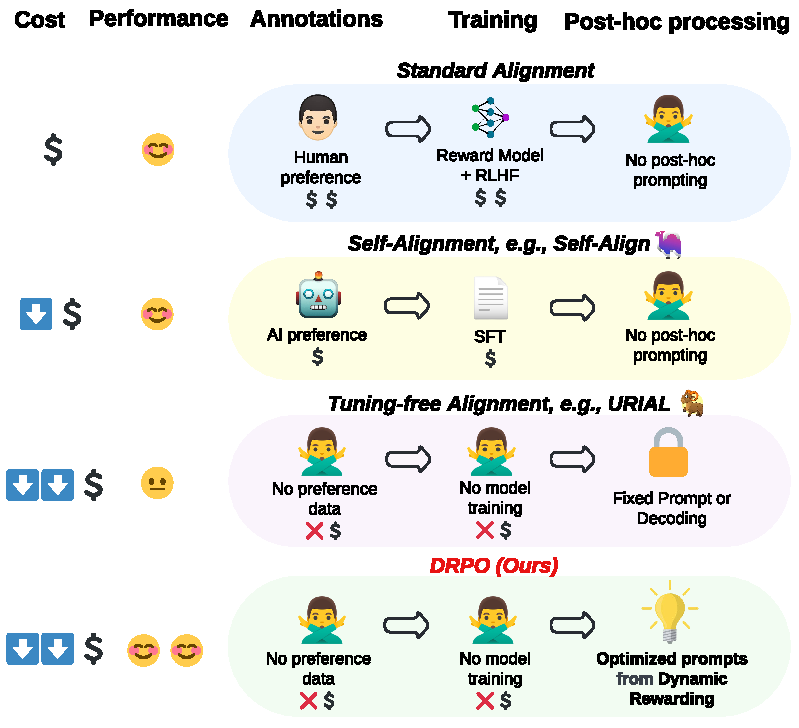
\includegraphics[width=1\linewidth]{images/DRPO_comparison.pdf}
    \vspace{-18pt}
    \caption{Comparison of \ours with other LLM alignment paradigms. \ours combines the benefits of self-alignment and tuning-free alignment, enabling self-improvement and high cost-efficiency without requiring human supervision or additional model training.
    }
    \vspace{-22pt}
    \label{fig:paradigm_comparison}
\end{figure}



Self-alignment aims to improve LLM alignment by leveraging the models themselves; for example, by replacing human feedback with model-generated feedback~\cite{lee2023rlaif}, synthesizing preference data~\cite{kim2023aligning, sun2024principle}, or self-critique~\cite{bai2022constitutional}. Despite these advancements, such methods still demand significant resources, including the costly and unstable RLHF tuning, as well as some level of human supervision, such as carefully curated alignment rules or in-context learning (ICL) prompts~\cite{sun2024principle}. On the other hand, as shown in Figure~\ref{fig:paradigm_comparison}, a recent line of research focuses on tuning-free alignment, which prioritizes extreme efficiency without incurring any tuning cost. These approaches include techniques like decoding-based alignment~\cite{li2023rain, wang2024inferaligner} or ICL alignment~\cite{han2023context, Lin2024ReAlign, zhao2024context}. However, these tuning-free methods are often static (e.g., relying on fixed prompts or reward functions) and thus lack the flexibility to adapt and self-improve for better alignment. 




To marry the strengths of both paradigms, in this paper, we propose \ours, Dynamic Rewarding with Prompt Optimization, a novel tuning-free approach for LLM self-alignment. \ours draws inspiration from two key insights from recent alignment research. First, the superficial alignment hypothesis~\cite{zhou2024lima} suggests that LLMs can be effectively aligned through lightweight tuning or even simple prompting~\cite{Lin2024ReAlign, zhao2024context}. Second, reward models in RLHF often generalize poorly to out-of-distribution samples~\cite{burns2023weak}, whereas LLMs, known for their superior generalization capabilities, can provide more effective rewards and feedback for alignment purposes. Building on these insights, \ours is constructed atop a search-based prompt optimization (PO) framework~\cite{pryzant2023automatic, hao2023reasoning, wang2023promptagent}, which enables LLMs to self-correct and automatically craft detailed alignment instructions. This steers model behavior more effectively, without relying on any use of human preferences or model training. 




The core novelty of \ours lies in its \textit{dynamic rewarding} mechanism, integrated with the optimization framework. This mechanism allows LLM-based rewards to be dynamically adjusted based on specific queries, helping to identify and address the model's alignment blind spots. For example, if an LLM with outdated knowledge pretends to answer a question requiring the latest news, its ``knowledge limitation'' reward will be low, and the alignment prompt will be updated accordingly. We apply this novel method to automatically craft both the system prompt and responses in ICL examples, which have proven highly effective in improving alignment.




We conducted comprehensive experiments on 8 recent LLMs using the standard alignment benchmark, \texttt{just-eval-instruct}, composed of questions from multiple alignment datasets. Our results show that \ours can effectively align both base and SFT/RLHF tuned models. Notably, \ours significantly enhances base models, enabling them to outperform their SFT/RLHF-tuned counterparts. \ours can further improve SFT/RLHF-tuned models, highlighting its compatibility with other tuning-based alignment techniques. Additionally, our automatically optimized prompts substantially outperform those curated by human experts. 





\begin{figure}
    \centering
    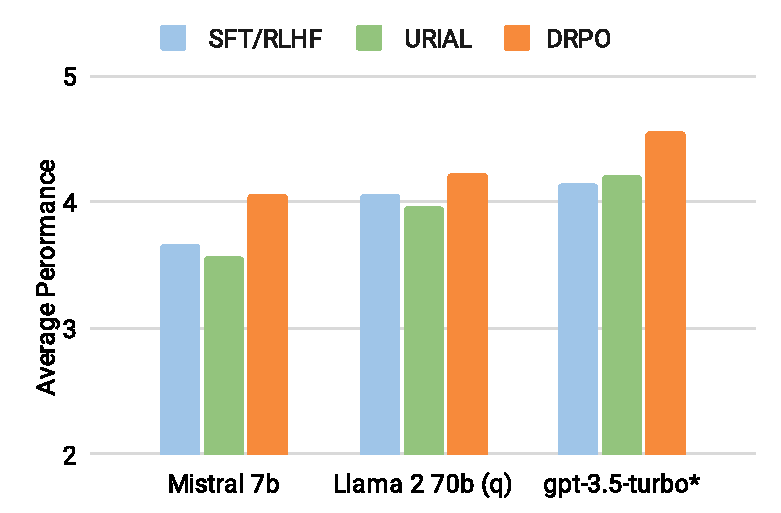
\includegraphics[width=1.0\linewidth]{images/method_comparison_column_chart_white_bg.pdf}
    \vspace{-15pt}
    \caption{Comparison of \ours with other alignment methods, including RLHF and URIAL~\cite{Lin2024ReAlign}. \ours consistently outperforms both baselines across multiple LLMs.
    Note that we do not have access to \texttt{gpt-3.5-turbo} base model; hence, both \ours and URIAL are directly applied to its RLHF-tuned version.}
    \label{fig:overall_comparison_chart}
    \vspace{-15pt}
\end{figure}













\section{Related Work}
\vspace{-5pt}


\noindent \textbf{Self-Alignment.}
Traditional alignment approaches rely heavily on extensive human-annotated preference data and complex reward model training through reinforcement learning, which poses significant scalability and cost challenges~\cite{ouyang2022training}. Self-alignment focuses on aligning LLMs themselves with model-generated feedback, datasets, critique, etc., which are then used for fine-tuning or training reward models~\cite{lee2023rlaif, bai2022training, cao2024towards, wang2024step, guo2024human}. Notable examples include synthesizing alignment training data with human-provided instructions and ICL examples~\cite{wang2022self, kim2023aligning, sun2024principle}, augmented web documents~\cite{li2023self}, or self-critique~\cite{bai2022constitutional, madaan2024self}. However, most of these methods still require an SFT/RLHF-tuning process to enhance alignment, along with some degree of human annotations or supervision. In contrast, \ours shares similar self-alignment principles using self-critique error feedback to gradually align the model, but it achieves this entirely without any model tuning or human supervision.



\begin{figure*}[ht]
    \centering
    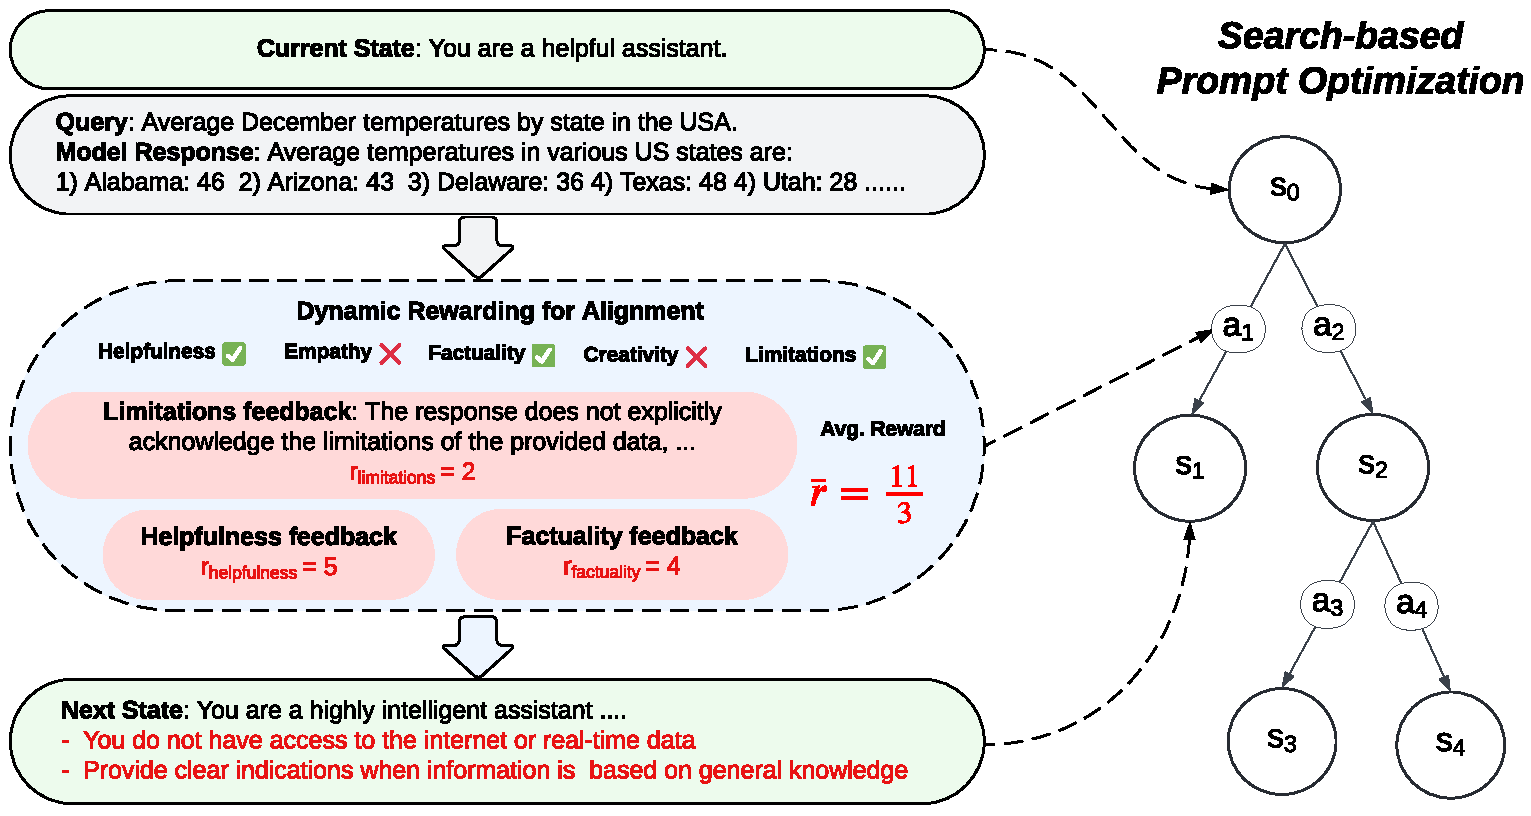
\includegraphics[width=0.95\linewidth]{images/Dynamic_Rewarding.pdf}
    \vspace{-8pt}
    \caption{Overall framework of Dynamic Rewarding with Prompt Optimization (\ours). The optimization problem is modeled as a Markov Decision Process (MDP) and solved using beam search to optimize the alignment prompt. Dynamic rewarding, a novel technique integrated into this framework, allows flexible reward assignment to detect and address alignment weaknesses in the current LLM, thereby enhancing the overall optimization process.
    }
    \label{fig:dynamic_rewarding}
    \vspace{-15pt}
\end{figure*}




\noindent \textbf{Tuning-Free Alignment.}
A recent trend in alignment research is to align LLMs without updating their parameters, typically as a post-training process for LLMs. This has witnessed two major lines of work recently. The first aligns models with carefully curated human annotations and ICL examples~\cite{han2023context, Lin2024ReAlign, zhao2024context}, while the second involves decoding-based methods to guide token generation and search with alignment rewards~\cite{li2023rain, khanov2024args, huang2024deal}. Although tuning-free, the first approach still requires human curation and often underperforms compared to SFT/RLHF-tuned counterparts. The second one, while effective, incurs higher inference costs per query, making it computationally expensive. It is worth mentioning that another recent promising direction is cost-efficient alignment through representation engineering~\cite{zou2023representation, wu2024reft}, which aims to steer LLM representation vectors for alignment~\cite{li2024inference, kong2024aligning, wang2024inferaligner}. However, these methods are not fully tuning-free and typically require additional data or model training to identify alignment directions in the embedding space. Nevertheless, \ours requires no additional annotations or model training, and also only needs a one-time optimization per model to achieve better performance than SFT/RLHF-tuned counterparts. 







\noindent \textbf{Prompt Optimization.}
Discovering optimal discrete prompts becomes far more crucial nowadays. Modern prompts for LLMs can be generally divided into two parts: in-context learning examples and detailed instructions. The former is usually treated as a retrieval problem with various schemas to select the influential examples~\cite{rubin2021learning, dong2022survey}. Optimizing the latter has been heavily studied recently, mostly formulated as a sampling or search problem. Generally, an initial prompt (e.g., a base prompt, ``You are a helpful assistant'') is given to start an iterative process, where diverse prompt candidates are generated per turn, and the best ones are kept for the next iteration. Various sampling strategies are proposed to diversify the prompt candidates, e.g., back translation~\cite{xu2022gps}, evolutionary operations~\cite{fernando2023promptbreeder}, self-critique~\cite{wang2023promptagent}. Different search frameworks also have been studied, such as Monte Carlo search~\cite{zhou2022large}, evolutionary algorithms~\cite{fernando2023promptbreeder, yang2023large}, beam search~\cite{pryzant2023automatic}, and Monte Carlo tree search (MCTS)~\cite{wang2023promptagent}. \ours builds upon recent search-based optimization methods but introduces novel techniques, such as dynamic rewarding, to effectively address the alignment problem. 
\section{Methodology}
\vspace{-5pt}


In this section, we introduce our formulation formally and present \ours for solving the alignment problem by optimizing the alignment instruction.

%Most existing methods for alignment use techniques like PPO \cite{Schulman2017ProximalPO} and DPO \cite{rafailov2023direct} which are very costly to execute as they need large amounts of data to be successful. 

% Most existing alignment methods, such as RLHF~\cite{ouyang2022training} and DPO~\cite{rafailov2023direct}, are generally expensive to execute, requiring not only large amounts of data but also substantial computational resources and human labeling efforts.
% Research on using in-context learning for alignment has been limited and primarily relies on human-generated prompts and in-context learning examples. To address this limitation, we introduce a systematic method to optimize prompts and in-context learning examples for LLMs without any human effort or annotation.


\subsection{Problem Formulation}

% \noindent \textbf{Problem Formulation}.
Given an LLM $\mathcal{B}$, an alignment instruction consists of two parts: a system prompt $\mathcal{P}$ and a set of $N$ in-context learning (ICL) examples $\mathcal{I}$.
The system prompt $\mathcal{P}$ serves as a prefix that provides high-level instructions, sets the tone, and imposes constraints on the model's responses. Each ICL example $\mathcal{I}_i$ consists of a pair $(q_i, d_i)$, where $q_i$ is an input query and $d_i$ is the corresponding desired response, so we can represent $\mathcal{I} = \{(q_1, d_1), (q_2, d_2), \ldots, (q_N, d_N)\}$. 

Conditioning on the system prompt $\mathcal{P}$ and a selected subset of $K$ ICL examples $\mathcal{I}_K \subseteq \mathcal{I}$, the aligned model response $y$ to an input $x$ is generated as:
\[
y = \mathcal{B}(x \mid \mathcal{P}, \mathcal{I}_K)
\]

\ours aims to optimize both system prompt $\mathcal{P}$ and ICL examples $\mathcal{I}_K$ to enhance alignment. This involves finding the best possible $\mathcal{P}^*$ and $\mathcal{I}_K^*$ that maximize the alignment of the model's responses. This optimization problem can be formulated as follows:
\[
(\mathcal{P}^*, \mathcal{I}_K^*) = \arg\max_{\mathcal{P}, \mathcal{I}_K} \mathbb{E}_{x \sim \mathcal{D}_x} \left[\mathcal{B}(x \mid \mathcal{P}, \mathcal{I}_K) \right]
\]
\noindent where $\mathcal{D}_x$ denotes the distribution of input queries, and the expectation $\mathbb{E}$ represents the alignment performance for responses based on specific metrics.


% We propose a two-step approach to the optimization problem: 
% \begin{enumerate}
%     \item Estimating $\mathcal{I}^*$ (universal).
%     \item Estimating $\mathcal{P}^*$ given ${\mathcal{I}}^*$. (model specific)
% \end{enumerate}


% \subsection{Systematic Optimization Framework}

% We approach the optimization of the system prompt $\mathcal{P}$ and in-context learning examples $\mathcal{E}$ using the unified framework LLM Reasoners~\cite{hao2024llm} that involves a base model $\mathcal{B}$, an optimizer $\mathcal{O}$, and an evaluator $\mathcal{E}$. This framework is treated as a search process that iteratively interacts with the model's environment and adjusts the prompt $\mathcal{P}$ based on a reward function $\mathcal{R}$. The main challenge for our problem is -the design of a reward function for a problem as broad and general as Alignment. To overcome this challenge we introduce `Dynamic Rewarding', which can effectively handle tasks as broad and challenging as alignment.


\subsection{Dynamic Rewarding with Prompt Optimization (\ours)}

Given the distinct nature of the system prompt and ICL examples, we propose to optimize them separately, resulting in a two-step optimization approach. We first construct a universal set of ICL examples and optimize their responses to obtain $\mathcal{I}^*$. Next, we estimate a model-specific system prompt $\mathcal{P}^*$ based on the optimized universal set $\mathcal{I}^*$. Notably, we leverage the \texttt{LLM Reasoners}\footnote{\url{https://github.com/maitrix-org/llm-reasoners}} framework~\cite{hao2023reasoning, hao2024llm} as the prompt optimization (PO) framework. Specifically, \texttt{LLM Reasoners} incorporates a base model $\mathcal{B}$, an optimizer $\mathcal{O}$, and an evaluator $\mathcal{E}$. It operates as a search agent that iteratively interacts with the model's environment, using the optimizer $\mathcal{O}$ to adjust the prompt $\mathcal{P}$ or ICL examples $\mathcal{I}$ based on a reward function $\mathcal{R}$. For further details, we refer readers to the original references. In the following, we introduce the core component of \ours. 


\subsubsection{Dynamic Rewarding for Alignment}

We formulate this optimization problem as a Markov Decision Process (MDP). In this framework, the states $s\in \mathcal{S}$ represent our optimization goal, which could be either a system prompt or an in-context example. Actions $a \in \mathcal{A}$ are defined based on the alignment feedback obtained during the evaluation of any given state. The key motivation is to leverage the superior generalization capabilities of LLMs to evaluate and analyze states, guiding state transitions toward an optimal state. We employ different evaluation techniques for system prompt and in-context example optimization, which are detailed in subsequent sections. Efficient traversal of this state space is crucial, and for this purpose, we adopt beam search due to its effectiveness and low computational cost.


One of the key challenges in our optimization task is designing a reward function capable of handling a problem as broad and generalized as alignment. As illustrated in Figure~\ref{fig:dynamic_rewarding}, a single, unified reward function is impractical due to the vast query space we aim to align with the base LLM $\mathcal{B}$. Different queries emphasize different focal points, meaning that certain evaluation criteria might be appropriate for some queries but not for others. To overcome this, we introduce a dynamic reward function $\mathcal{R}$, which can dynamically adapt to the specific query being evaluated. Notably, our approach shares conceptual similarities with a few recent alignment research, which also advocate for adaptable and query-sensitive alignment strategies~\cite{bai2022constitutional, sun2024principle}. However, the key distinction lies in our dynamic reward function’s ability to not only enable flexible evaluation but also integrate seamlessly into a formally defined optimization framework.



Specifically, we first predefined a set of reward criteria $\mathbb{R}$, from which the model dynamically selects the most relevant rewards, while also retaining the flexibility to propose new ones when necessary. Formally, for a given query \( q \), the dynamic reward function $\mathcal{R}$ evaluates the model's response $\sigma$ based on a dynamically selected or proposed rewards $\mathbb{R}_q$, where $\mathbb{R}_q \subseteq \mathbb{R} \cup \mathbb{R}^*$ and $\mathbb{R}^*$ represents newly proposed rewards. The reward function is defined as:

\[
\mathcal{R}(\sigma \mid \mathbb{R}_q) = \frac{1}{|\mathbb{R}_q|} \sum_{r \in \mathbb{R}_q} r(\sigma)
\]

Here, $\mathbb{R}_q$ denotes relevant rewards tailored for the given query \( q \) and \(r(\sigma)\) denotes the score of a specific reward when evaluating any response \(\sigma\). 

This allows us to flexibly score and evaluate responses based on the most relevant criteria for each specific query, ensuring that the evaluation remains contextually appropriate and comprehensive.




\subsubsection{ICL Example Optimization}

To optimize in-context learning examples, we start with a set of base ICL examples $\mathcal{I}_{\text{base}} = \{(q_1, b_1), (q_2, b_2), \ldots, (q_N, b_N)\} $, where $q_i$ is a query and $b_i$ is a base response to the query, $N$ is the total number of in-context examples. Our overall goal is to find a universal set $\mathcal{I}^{*}$ that maximizes alignment across various models.


We specifically optimize each ICL example $(q_i, b_i)$ individually. The initial state of the search tree for an ICL example is defined as the base response to the query, i.e.,  $s_0 = b_i$. At any time $t$, the state of the search tree, $s_t$, is the response of the example. This allows us to systematically monitor and evaluate the response at any given time $t$. The state space $\mathcal{S}$ encompasses all possible responses to the query $q_i$.


To evaluate and improve the alignment, we use the dynamic reward function $\mathcal{R}$. The relevant rewards $\mathbb{R}_{q_i}$ for the query $q_i$ are specifically selected or potentially proposed new rewards. The reward function $\mathcal{R}$ and evaluator $\mathcal{E}$ then evaluates the state $s_t$ based on these rewards, providing a reward $r_t$ and alignment feedback $a_t$:

\[
\begin{aligned}
& r_t = \mathcal{R}(s_t \mid \mathbb{R}_{q_i}) \\
& a_t = \mathcal{E}(s_t \mid \mathbb{R}_{q_i})
\end{aligned}
\]

Note that, in practice, evaluation and reward generation are performed simultaneously using one single prompt, so the evaluation can also be considered dynamic. The transition function $\mathcal{T}$, implemented by optimizer $\mathcal{O}$, then updates the state:
\[
s_{t+1} = \mathcal{T}(s_t, a_t)
\]

The detailed pseudo-code for this optimization process is provided in Algorithm \ref{alg:icl_opti} in Appendix \ref{sec:opti_algo} and the prompts used by our algorithm can be found in Appendix \ref{sec:meta_prompts}.



\subsubsection{System Prompt Optimization}

The optimization process for the system prompt is similar to that of the ICL example optimization. For the system prompt optimization, we use $K$ optimized ICL examples $\mathcal{I}_K^*  \subseteq \mathcal{I}^*$, where the $K$ ICL examples are chosen using similarity-based retrieval. We collect a set of seed samples $\mathcal{X} = \{x_1, x_2, \ldots, x_N \}$, where $x_i$ is a query that will be used to test the alignment of the base model $\mathcal{B}$. The goal of this process is to find the optimal prompt $\mathcal{P}^*$ (given that we already have access to $\mathcal{I}_K^*$), such that alignment of LLM $\mathcal{B}$ is maximized. This prompt is specific to the base model $\mathcal{B}$ and will provide the model with actionable insights and guidance to improve its alignment.


The optimization process begins by defining the initial state $s_0$ as the basic system prompt (e.g., ``You are a helpful assistant.''). At any time $t$, the state $s_t$ represents the current system prompt, and the state space $\mathcal{S}$ includes all possible system prompts for the given LLM $\mathcal{B}$.


For a given state $s_t$, we sample a query $x_t$ from the seed samples $\mathcal{X}$. The relevant rewards $\mathbb{R}_{x_t}$ for the query $x_t$ are specifically selected or potentially proposed new rewards. The reward function $\mathcal{R}$ and the evaluator $\mathcal{E}$ then evaluate the response generated by the model $\mathcal{B}$ given the system prompt $s_t$ and the selected in-context examples $\mathcal{I}_K^*$, providing a reward $r_t$ and alignment feedback $a_t$:

\[
\begin{aligned}
& r_t = \mathcal{R}(\mathcal{B}(x_t \mid s_t, \mathcal{I}_K^*)\mid \mathbb{R}_{x_t}) \\
& a_t = \mathcal{E}(\mathcal{B}(x_t \mid s_t, \mathcal{I}_K^*)\mid \mathbb{R}_{x_t})
\end{aligned}
\]

The optimizer $\mathcal{O}$ as a transition function then updates the state, $ s_{t+1} = \mathcal{T}(s_t, a_t) $. The detailed pseudo-code for this optimization process is provided in Algorithm \ref{alg:prompt_opti} in Appendix \ref{sec:opti_algo}.
\section{Experiments}


\subsection{Experimental Setup}


% main table comparing the baselines and our own methods

\begin{table*}[t]
\begin{center}
\begin{tabular}{ >{\raggedright\arraybackslash}p{3.9cm} c c c c c c c c } 
    \toprule

    \textbf{[Tuned] Model} & \textbf{Method }& \bm{$K$} & \textbf{Helpful} & \textbf{Clear} & \textbf{Factual} & \textbf{Deep} & \textbf{Engage} & \textbf{Avg.} \\
    \midrule

    [\xmark] Mistral 7b  & Base & 0 & 2.20 & 2.51 & 2.29 & 1.69 & 1.80 & 2.10 \\
    
   [\xmark] Mistral 7b  & URIAL & 3 & 3.62 & 4.32 & 3.75 & 2.70 & 3.41 &  3.56\\
    
    [\xmark] Mistral 7b  & \ours & 2 & \textbf{4.23} & \textbf{4.56} & \textbf{3.97} & \textbf{3.68} & \textbf{3.84} &  \textbf{4.06}\\
    
    \hline
    
   [\cmark] Mistral 7b (Instruct) & Base & 0 & 3.98 & 4.44 & 3.64 & 2.97 & 3.26 &  3.66\\
    
   [\cmark] Mistral 7b (Instruct) & URIAL & 3 & 3.94 & 4.51 & 3.69 & 2.99 & 3.75 &  3.78\\
    
    [\cmark] Mistral 7b (Instruct) & \ours & 2 & \textbf{4.22} & \textbf{4.60} & \textbf{3.80} & \textbf{3.68} & \textbf{3.99} &  \textbf{4.06}\\

   \hline

    [\xmark] Llama 2 70b$^q$  & Base & 0 & 2.07 & 2.55 & 2.35 & 1.50 & 1.63 &  2.02 \\
    
    [\xmark] Llama 2 70b$^q$ & URIAL & 3 & 4.25 & 4.67 & 4.03 & 3.08 & 3.80 &  3.97 \\
    
    [\xmark] Llama 2 70b$^q$  & \ours & 2 & \textbf{4.42} & \textbf{4.72} & \textbf{4.23} & \textbf{3.81} & \textbf{3.98} &  \textbf{4.23}\\

    \hline

    [\cmark] Llama 2 70b$^q$ (chat) & Base & 0 & 4.36 & 4.71 & 3.95 & 3.56 & 3.76 &  4.07\\

    [\cmark] Llama 2 70b$^q$ (chat) & URIAL & 3 & 4.32 & 4.72 & 4.08 & 3.50 & 4.25 &  4.17\\
    
    [\cmark] Llama 2 70b$^q$ (chat) & \ours & 2 & \textbf{4.46} & \textbf{4.75} & \textbf{4.10} & \textbf{4.11} & \textbf{4.37} &  \textbf{4.36}\\


   \hline

    [\xmark] Llama 3 8b  & Base & 0 & 1.82 & 2.27 & 2.20 & 1.38 & 1.48 &  1.83\\

    [\xmark] Llama 3 8b  & URIAL & 3 & 3.94 & \textbf{4.51} & 3.69 & 2.99 & \textbf{3.75} & 3.78 \\
    
    [\xmark] Llama 3 8b  & \ours & 2 & \textbf{4.02} & 4.40 & \textbf{3.84} & \textbf{3.50} & 3.65 &  \textbf{3.88} \\

   \hline

    [\cmark] Llama 3 8b (Instruct) & Base & 0 & 4.43 & 4.72 & 3.98 & 3.45 & 3.76 &  4.07\\

    [\cmark] Llama 3 8b (Instruct) & URIAL & 3 & 4.48 & 4.81 & \textbf{4.19} & 3.55 & 4.27 &  4.26\\
    
    [\cmark] Llama 3 8b (Instruct) & \ours & 2 & \textbf{4.54} & \textbf{4.81} & 4.16 & \textbf{4.08} & \textbf{4.40} & \textbf{4.40} \\

    \hline

    [\cmark] \texttt{gpt-3.5-turbo} & Base & 0 & 4.56 & 4.89 & 4.41 & 3.30 & 3.55 & 4.14 \\

    [\cmark] \texttt{gpt-3.5-turbo} & URIAL & 3 & 4.30 & 4.77 & 4.41 & 3.44 & 4.11 &  4.21\\
    
    [\cmark] \texttt{gpt-3.5-turbo} & \ours & 2 & \textbf{4.67} & \textbf{4.92} & \textbf{4.53} & \textbf{4.07} & \textbf{4.58} &  \textbf{4.55}\\

   \hline
    [\cmark] \texttt{gpt-4-0613} & Base & 0 & \textbf{4.71} & \textbf{4.93} & \textbf{4.52} & 3.49 & 3.53 &  \textbf{4.24} \\

    \bottomrule

\end{tabular}

\caption{Performance on \texttt{just-eval-instruct} benchmark. ``Tuned'' indicates whether the model has been SFT/RLHF tuned. Models are evaluated across multiple aspects: ``Helpful'' (Helpfulness), ``Clear'' (Clarity), ``Factual'' (Factuality), ``Deep'' (Depth), and ``Engage'' (Engagement). The base method indicates a basic alignment prompt. Our method consistently outperforms baseline methods across multiple aspects and overall.}
\label{tab:main_table}
\vspace{-17pt}
\end{center}
\end{table*}


\noindent \textbf{Evaluation Dataset}.
We use the standard alignment benchmark, \texttt{just-eval-instruct}~\cite{Lin2024ReAlign}, which merges five popular alignment datasets to provide a comprehensive and fine-grained evaluation of LLM alignment. This benchmark consists of 1,000 examples: the first 800 assess the models' helpfulness, and the remaining 200 evaluate their harmlessness. The first 800 examples are evaluated based on five fine-grained aspects: \textit{helpfulness}, \textit{clarity}, \textit{factuality}, \textit{depth}, and \textit{engagement}, while the remaining 200 are evaluated using the \textit{safety} aspect. We use GPT-4 Turbo (\texttt{gpt-4-1106-preview}), one of the latest GPT-4 models available during our experiments, to evaluate both types of examples using the prompts specified in the original URIAL paper~\cite{Lin2024ReAlign}. The scoring scale ranges from 1 to 5, indicating ``strongly disagree'', ``disagree'', ``neutral'', ``agree'', and ``strongly agree''. Note that we employ a more recent version of GPT-4 compared to URIAL, which enhances the strictness and accuracy of our evaluation pipeline. Thus, we re-benchmark URIAL under our updated evaluation setting for consistency across all results.


\noindent \textbf{Seed Samples}. 
When optimizing the system prompt with \ours, we sample from our seed dataset $\mathcal{X}$ to measure the alignment performance of the system prompt at each time step. This seed dataset, consisting of 180 examples, is built using data from \texttt{AlpacaEval} \cite{alpaca_eval}, \texttt{LIMA} \cite{zhou2024lima}, and \texttt{HH-RLHF-redteam} \cite{Ganguli2022RedTL}. More details about the construction of this dataset can be found in Appendix \ref{sec:impl_details}.


\noindent \textbf{Models}.
We benchmark 6 open-source LLMs in our experiments: Mistral 7b (v0.1), Mistral 7b (Instruct)~\cite{Jiang2023Mistral7}, Llama 2 70$b^q$, Llama 2 70$b^q$ (chat) (4-bit AWQ~\cite{lin2023awq} quantized models)~\cite{Touvron2023Llama2O}, Llama 3 8b, Llama 3 8b (Instruct)~\cite{llama3modelcard} and 2 closed-source models: OpenAI's GPT-3.5 Turbo (\texttt{gpt-3.5-turbo}) and GPT-4 (\texttt{gpt-4-0613}). Models without the ``chat'' or ``instruct'' tag are base models, i.e., not tuned by SFT/RLHF. For evaluation, we use greedy decoding (temperature = 0) to ensure reproducibility.



\noindent \textbf{Baselines}. 
We first apply \ours to the base model, making the SFT/RLHF-tuned counterparts without \ours a natural baseline. For instance, we compare Mistral 7B + \ours and Mistral 7b (Instruct). Additionally, we have two more baselines: (1) The base method, where a basic prompt is applied without using ICL examples. (2) URIAL~\cite{Lin2024ReAlign}, where we use the prompt and ICL examples proposed by authors. We also provide extensive ablation baselines of our method, such as changing the search algorithm from Beam search to Greedy Search or Monte Carlo search and using ``static rewarding'' to understand the impact of dynamic rewarding. Full details of these can be found in Appendix~\ref{sec:impl_details}.




\noindent \textbf{Implementation details}.
We use GPT-4-turbo (\texttt{gpt-4-0125-preview}) as both the optimizer $\mathcal{O}$, and evaluator $\mathcal{E}$ unless specified otherwise. The initial set of in-context learning examples, $\mathcal{I}_{base}$, contains 16 examples: 3 from URIAL \cite{Lin2024ReAlign} and 13 generated using \texttt{gpt-4-0125-preview}. More details about the design choice made for $\mathcal{I}_{base}$ can be found in Appendix \ref{sec:impl_details}. We employ sentence transformers \cite{reimers-2019-sentence-bert} to retrieve K in-context learning examples from $\mathcal{I}^*$ given the query. We use $D$ as the beam depth, $W$ as the beam width, and $M$ as the number of action samples per state (to grow the tree for the next iteration). The exact hyper-parameters can be found in Appendix \ref{sec:impl_details}.


\subsection{Results}

\noindent \textbf{Comparison with baselines}. 
Table \ref{tab:main_table} presents the performance comparison of \ours with baselines. \ours outperforms all baselines across both tuned and un-tuned models. As shown in Figure \ref{fig:overall_comparison_chart} using \ours on strong base models such as Mistral 7b and LLama 2 70b$^q$ can surpass even the RLHF/SFT tuned models under base setting. It is noteworthy that \ours achieves superior performance compared to URIAL \citep{Lin2024ReAlign}, despite using fewer in-context learning examples, highlighting the quality of optimized alignment instruction by \ours. Note that while \texttt{just-eval-instruct} includes a \textit{safety} metric, we are not reporting it because, in our analysis, we found that the safety metric is saturated, with all methods (RLHF/SFT, URIAL, and \ours) achieving consistently high scores. This saturation is a good sign, demonstrating that tuning-free methods like \ours can result in very safe models that adhere to human values.



\noindent \textbf{Categorized performance}. 
Appendix~\ref{sec:cat_perf} presents the performance of models across various domains, e.g., ``procedure'', ``lifestyle'', ``info-seek'', ``STEM'', etc. In this experiment, we apply \ours to base models and compare their performance across multiple human-relevant and alignment-critical domains. \ours demonstrates consistently strong performance, surpassing RLHF/SFT-tuned models in most domains across all baselines.




\begin{table}[!t]
\begin{center}
\begin{tabular}{ c c c c } 
    \toprule
    \multirow{2}{*}{\textbf{Model}} & \textbf{Mistral}  & \textbf{Llama}  & \textbf{Base} \\
    & \textbf{Prompt} & \textbf{Prompt} & \textbf{Prompt} \\
    \midrule
    Mistral 7b & \textbf{4.06} & 4.03 & 4.04 \\
    Llama 2 70$b^q$ & 4.19 & \textbf{4.23} & 4.17 \\
    \bottomrule
\end{tabular}
\caption{Effect of prompt transfer on base LLMs. The best performance is achieved when using a prompt specifically optimized for the target base LLM.}
\label{tab:prompt_transfer}
\vspace{-17pt}
\end{center}
\end{table}
% Prompt Transfer table
\noindent \textbf{Prompt transfer}. 
We also conduct experiments on prompt transfer, i.e., evaluating the performance of an alignment instruction optimized for one LLM on a different LLM. Table~\ref{tab:prompt_transfer} presents the results of transferring various optimized prompts to Mistral 7b and Llama 2 70$b^q$. While the best results are achieved with prompts specifically optimized for the target model, transferring an optimized prompt can still lead to significant alignment improvements. This is evident in the case of LLaMA 2 70B$^q$, which benefits from the prompt optimized for Mistral 7B.





\noindent \textbf{Ablation on system prompt and  ICL examples}. 
Table \ref{tab:ablation_icl_prompt} shows the effect of ablating system prompt and in-context learning examples from \ours. Using both system prompt and in-context learning examples gave the best performance, underscoring the importance of both in alignment. It is worth pointing out that performance degradation on the removal of in-context learning examples was higher when compared to the removal of the system prompt, hinting that in-context learning examples are relatively important in alignment. Given this, our optimized in-context learning examples are a valuable asset and will be released publicly to facilitate further alignment research\footnote{\url{https://github.com/Singla17/DRPO}}.

\begin{table}[!t]
\begin{center}
\resizebox{0.9\linewidth}{!}{%
\begin{tabular}{ c c c c } 
 \toprule
 \multirow{2}{*}{\textbf{Model}} & \textbf{System} & \textbf{ICL} & \multirow{2}{*}{\textbf{Avg.}} \\
 & \textbf{Prompt} & \textbf{(}\bm{$K = 2$}\textbf{)} &  \\
 \midrule

  Mistral 7b  & \cmark & \cmark & \textbf{4.06} \\
 Mistral 7b (Instruct) & \cmark & \cmark & \textbf{4.06} \\
 Llama 2 70$b^q$  & \cmark & \cmark & \textbf{4.23} \\
 \texttt{gpt-3.5-turbo} & \cmark & \cmark & \textbf{4.55} \\

 \midrule


  Mistral 7b & \xmark & \cmark & 4.04 \\
 Mistral 7b (Instruct) & \xmark & \cmark & 4.04 \\
 Llama 2 70$b^q$  & \xmark & \cmark & 4.17 \\
 \texttt{gpt-3.5-turbo} & \xmark & \cmark & 4.42 \\

  \midrule


 Mistral 7b (Instruct) & \cmark & \xmark & 3.67 \\
 Llama 2 70$b^q$  & \cmark & \xmark & 3.63 \\
 \texttt{gpt-3.5-turbo} & \cmark & \xmark & 4.34 \\

  \bottomrule

\end{tabular}
}
\caption{Ablation study on the impact of removing the optimized system prompt and in-context learning (ICL) examples optimized using our method. In the absence of the optimized system prompt, a basic system prompt is provided. Our method consistently outperforms all ablation variants across all models.}
\label{tab:ablation_icl_prompt}
\vspace{-20pt}
\end{center}
\end{table}


% Search Algo Ablation table
\noindent \textbf{Ablation on search algorithms}. 
Table \ref{tab:ablation_search_algo} presents the effect of search algorithms on prompt optimization. We have kept the state and action definitions the same and have only changed the underlying search algorithm.  In this experiment, we ensured that MC and Beam sample the same number of prompts, i.e., same cost, whereas greedy search has a lower cost because the beam width is fixed at 1. More implementation details can be found in Appendix \ref{sec:impl_details}. \ours with beam search gives the best results, depicting the need for thoughtful search and efficient optimization for optimal results.

\begin{table}[!t]
\begin{center}

\begin{tabular}{ c c c  } 
    \toprule
    \textbf{Model} & \textbf{Search} & \textbf{Avg.} \\
    % \multirow{2}{*}{Model} & Prompt &  \multirow{2}{*}{Avg.} \\
    % & Search &  \\
    
    \midrule
    Mistral 7b (Instruct) & Beam  & \textbf{4.06} \\
    \midrule
    
    Mistral 7b (Instruct) &  MC  & 4.02 \\
    Mistral 7b (Instruct) & Greedy & 4.02 \\
    
    \bottomrule
    
\end{tabular}

\caption{Ablation study on search methods. MC: Monte Carlo Search; Greedy: greedy search; Beam: beam search. Our method outperforms all other search algorithms tested in the ablation study.}
\vspace{-10pt}
\label{tab:ablation_search_algo}
\end{center}
\end{table}




% Methodological Ablation table


\begin{table}[!t]
\begin{center}
\resizebox{0.9\linewidth}{!}{%
\begin{tabular}{ c c c c } 
    \toprule
    \multirow{3}{*}{\textbf{Model}} & \textbf{Dynamic} &  \textbf{Dynamic}  &\multirow{3}{*}{\textbf{Avg.}} \\
    & \textbf{Reward} &  \textbf{Reward } \\
    & \textbf{Prompt} & \textbf{ICL} \\
    
    \midrule
    Mistral 7b (Instruct) & \cmark  & \cmark & \textbf{4.06} \\
    \midrule 
    
    Mistral 7b (Instruct) &  \xmark  & \cmark  & 4.02 \\
    Mistral 7b (Instruct) & \cmark & \xmark & 3.86 \\

    \bottomrule
    
\end{tabular}}

\caption{Ablation study on dynamic rewarding, examining its removal from system prompt and ICL example optimization. Our method, utilizing dynamic rewarding for both prompts and ICL examples, consistently outperforms both ablation variants.}
\label{tab:ablation_method}
\end{center}
\vspace{-20pt}
\end{table}


\noindent \textbf{Ablation on dynamic rewarding}.
We performed ablations on the dynamic rewarding mechanism. Table \ref{tab:ablation_method} depicts that \ours, with its current setting of using dynamic rewards for system prompt and ICL optimization, works the best. The in-context examples and prompts without using Dynamic rewarding are also optimized by `static rewarding' for a fair comparison, i.e., we ask the Optimizer to optimize all the rewards all the time. More details can be found in Appendix \ref{sec:impl_details}. 



\noindent \textbf{Effect of the number of in-context examples}.
Figure \ref{fig:icl_variation_chart} visualizes the effect of changing the number of in-context learning examples on alignment performance. The choice of $K = 2$ resulted in the best overall performance for Mistral 7b, ensuring strong alignment at a lower context length cost. Also, as observed in Figure \ref{fig:icl_variation_chart}, higher $K$ does not necessarily improve performance, hinting that the quality of ICL examples is more important. The importance of quality is also highlighted in Table \ref{tab:main_table}, where \ours outperforms URIAL at a lower $K$.


% ICL variation line chart
\begin{figure}[!t]
    \centering
    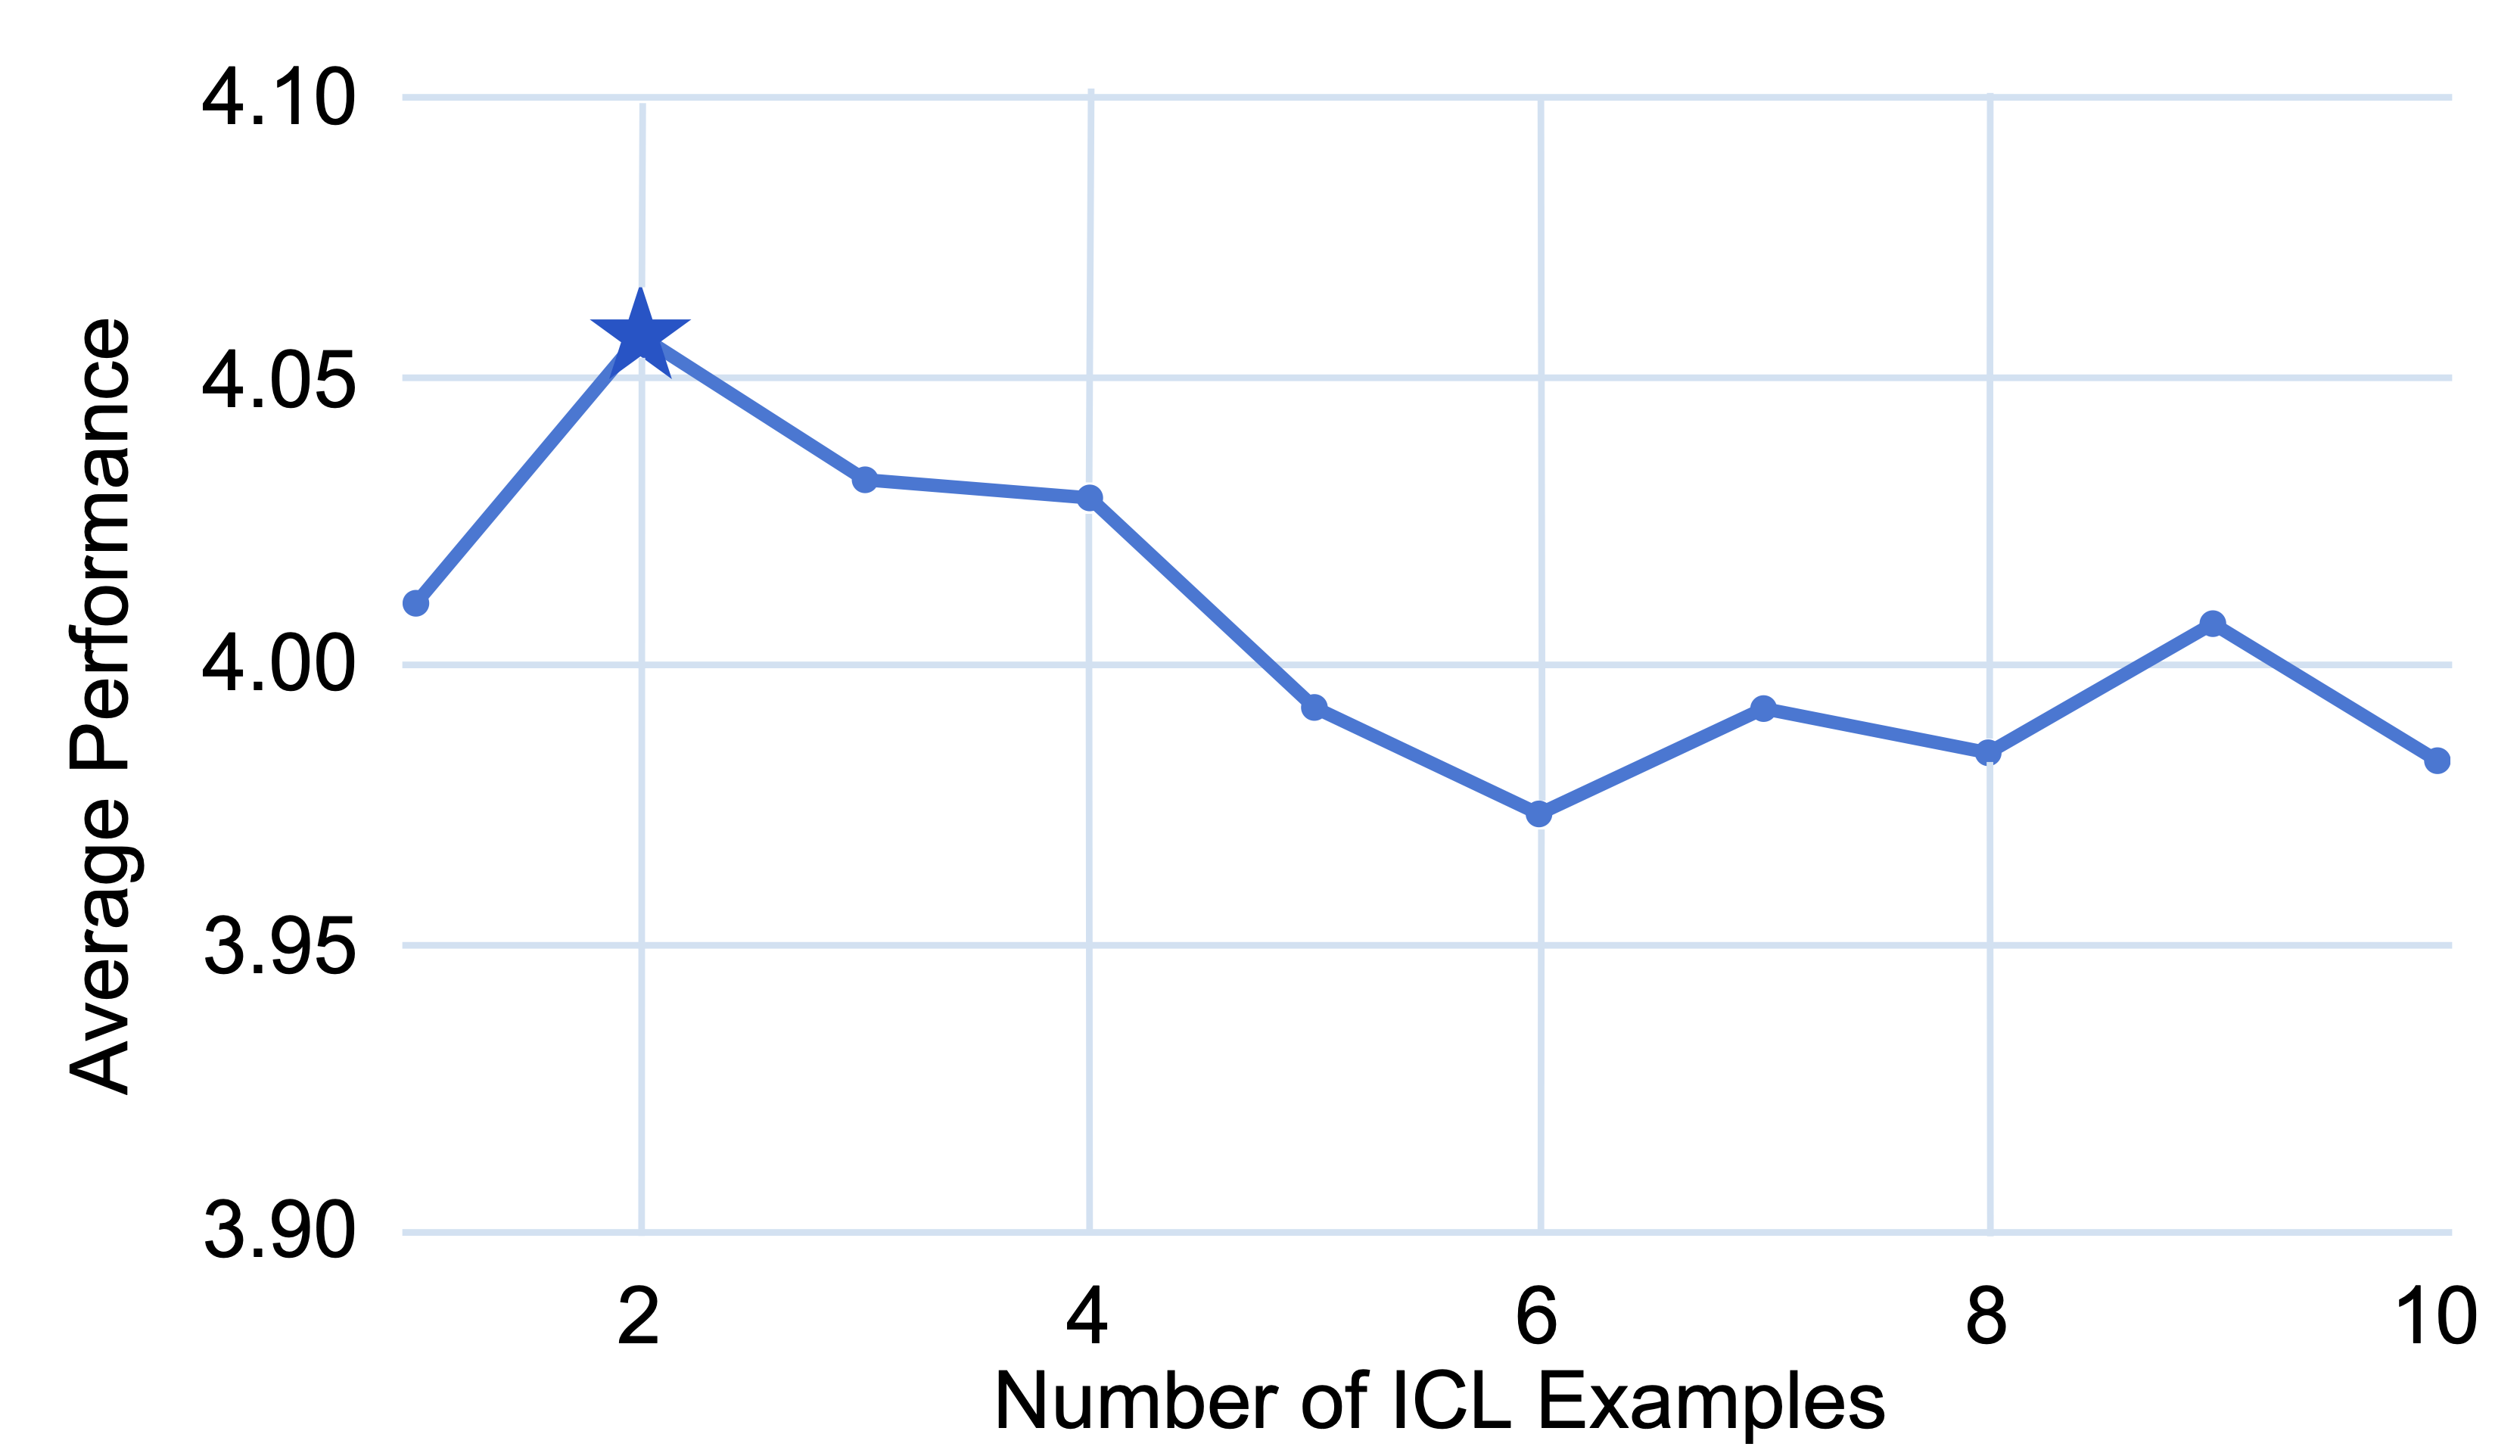
\includegraphics[ width=\linewidth]{images/icl_variation_line_chart_white_bg_v2.png}
    \caption{Performance of Mistral 7b (Instruct)  on varying the number of ICL examples. Two examples give us the best performance with a lower context length cost.}
    \label{fig:icl_variation_chart}
    \vspace{-5pt}
\end{figure}



% Qualitative analysis of gpt prompt

\newcommand{\reduline}[1]{{\color{red}\underline{{\color{black}#1}}}}

\newcommand\dunderline[2][.2pt]{\raisebox{-#1}{\underline{\raisebox{#1}{\smash{\underline{#2}}}}}}

\begin{table}[!t]

\definecolor{Gray}{gray}{0.90}
\newcolumntype{a}{>{\columncolor{Gray}}c}
\centering
\resizebox{1\linewidth}{!}{%
\begin{tabular}{@{}p{10cm}@{}}
\toprule
\textbf{Optimized Alignment Prompt} \\
\midrule
As a helpful and ethical assistant, your primary goal is to provide responses that are accurate, engaging, clear, and emotionally resonant across a wide range of queries. \\
- \ctext[RGB]{230,246,255}{Strive to make complex topics understandable and emotionally engaging, communicating in a human-like and relatable manner. Organize your responses to enhance readability and emotional connection, avoiding overly technical jargon.}  \\
- \ctext[RGB]{233,252,232}{Always acknowledge the limitations of your knowledge, especially when speculating about historical 'what-ifs', future predictions, or interpreting emotions.} \\
- \ctext[RGB]{255,225,255}{Aim for a balance between detailed, informative content and a conversational, engaging tone. Incorporate storytelling elements, examples, analogies, and direct questions to make information relatable.} \\
- \ctext[RGB]{230,246,255}{Avoid overwhelming the user with excessive information; structure your responses to be clear, well-organized, and mindful of the user's cognitive load.}
 \\

 \bottomrule
\end{tabular}%
}
 
\caption{Snippets from the system prompt optimized for \texttt{gpt-3.5-turbo}. The optimized prompt clearly demonstrates improved alignment, addressing potential weaknesses in the model.}
\label{tab:gpt_prompt}
\vspace{-15pt}
\end{table}
\noindent \textbf{Qualitative analysis of optimized prompts}. 
We finally present qualitative results to show \ours' ability to identify a model's alignment weaknesses and tailor system prompts to address them, as shown in Table \ref{tab:gpt_prompt} for \texttt{gpt-3.5-turbo}. The color-coded text in the table highlights specific weaknesses of \texttt{gpt-3.5-turbo} identified by \ours, along with actionable insights. Notably, it highlights \ctext[RGB]{233,252,232}{knowledge limitations of the model}, \ctext[RGB]{255,225,255}{tips to improve engagement} and \ctext[RGB]{230,246,255}{technical verbiage}. For a weaker model like Mistral 7b, \ours identifies the problem of repetitive tokens, which is absent in a strong model like \texttt{gpt-3.5-turbo}. Complete optimized prompts for both models, along with detailed annotations on the differences, can be found in Appendix \ref{sec:prompt_case_study}.  

% radar chart, analyzing various domains/dimensions 

\section{Conclusion}\label{sec:conclusion}

In this study, we comprehensively analyzed the performance of six state-of-the-art LLMs on problems from the USAMO 2025 competition. Using a rigorous human evaluation setup, we found that all evaluated models performed very poorly, with even the best-performing model achieving an average accuracy of less than $25\%$. Through detailed examination of the models' reasoning traces, we identified several critical failure modes, including significant artifacts arising from the optimization strategies employed during model training. These findings underscore the substantial limitations of current LLMs in the rigorous mathematical reasoning required for high-level olympiad competitions, highlighting the need for substantial improvements in  proof generation capabilities.


% \section*{Acknowledgments}

% This document has been adapted
% by Steven Bethard, Ryan Cotterell and Rui Yan
% from the instructions for earlier ACL and NAACL proceedings, including those for
% ACL 2019 by Douwe Kiela and Ivan Vuli\'{c},
% NAACL 2019 by Stephanie Lukin and Alla Roskovskaya,
% ACL 2018 by Shay Cohen, Kevin Gimpel, and Wei Lu,
% NAACL 2018 by Margaret Mitchell and Stephanie Lukin,
% Bib\TeX{} suggestions for (NA)ACL 2017/2018 from Jason Eisner,
% ACL 2017 by Dan Gildea and Min-Yen Kan,
% NAACL 2017 by Margaret Mitchell,
% ACL 2012 by Maggie Li and Michael White,
% ACL 2010 by Jing-Shin Chang and Philipp Koehn,
% ACL 2008 by Johanna D. Moore, Simone Teufel, James Allan, and Sadaoki Furui,
% ACL 2005 by Hwee Tou Ng and Kemal Oflazer,
% ACL 2002 by Eugene Charniak and Dekang Lin,
% and earlier ACL and EACL formats written by several people, including
% John Chen, Henry S. Thompson and Donald Walker.
% Additional elements were taken from the formatting instructions of the \emph{International Joint Conference on Artificial Intelligence} and the \emph{Conference on Computer Vision and Pattern Recognition}.

% Bibliography entries for the entire Anthology, followed by custom entries
%\bibliography{anthology,custom}
% Custom bibliography entries only
\bibliography{main}

\appendix

\appendix


% \vskip 0.2cm
\section{Experimental Settings}
\label{section:reproduce}

% \vskip -0.2cm
\paragraph{Supervised image classification.} For all supervised classification experiments on ImageNet-1K, we follow the training recipes from ConvNeXt \citep{convnext}.
For ConvNeXt-B and ConvNeXt-L, we use the original hyperparameters without modification.
ViT-B and ViT-L models use the same hyperparameters as ConvNeXt-B, except that for ViT-L, the beta parameters for AdamW are set to (0.9, 0.95), and the stochastic depth rates are set to 0.1 for ViT-B and 0.4 for ViT-L. 

% \vskip 0.2cm
\paragraph{Diffusion models.} We use the official implementation~\citep{dit} for training all DiT models. We find that the default learning rate is suboptimal for the models considered in this paper. To address this, we conduct a simple learning rate search with the LN models and apply the tuned learning rates directly to the DyT models. We also observe that the zero initialization negatively affects the performance of DyT models. Therefore, we retain the zero initialization for LN models but remove the zero initialization for DyT models.

% \vskip 0.2cm
\paragraph{Large Language Models.} In our implementation of LLaMA models~\citep{touvron2023llama, touvron2023llama2, dubey2024llama} with DyT, we introduce an additional learnable scalar parameter immediately after the embedding layer, before any Transformer blocks. We initialize it to the square root of the model embedding dimension $\sqrt{d}$. Without this scaling scalar, we find that the magnitudes of model activations at the beginning of training are too small, and the training struggles to progress. The issue is mitigated by incorporating a learnable scalar, and the model can converge normally. This addition of a scalar is similar to the original Transformer~\citep{vaswani2017attention} design, which uses a fixed scalar of the same value at the same position.

We train all our LLaMA models on the Pile dataset~\citep{pile}. We use the codebase from \texttt{FMS-FSDP} \citep{fms-fsdp}, which provides a default training recipe for the 7B model that closely follows the LLaMA 2 paper~\citep{touvron2023llama2}. We maintain the learning rate at the default 3e-4 for 7B and 13B and 1.5e-4 for 34B and 70B, in line with LLaMA 2.
The batch size is set to 4M tokens
and each model is trained on a total of 200B tokens.


For evaluation, we test the pretrained models on 15 zero-shot commonsense reasoning tasks from \texttt{lm-eval} \citep{eval-harness}: \texttt{anli\_r1}, \texttt{anli\_r2}, \texttt{anli\_r3}, \texttt{arc\_challenge}, \texttt{arc\_easy}, \texttt{boolq}, \texttt{hellaswag}, \texttt{openbookqa}, \texttt{piqa}, \texttt{record}, \texttt{rte}, \texttt{truthfulqa\_mc1}, \texttt{truthfulqa\_mc2}, \texttt{wic}, and \texttt{winogrande}. The selection closely follows that of OpenLLaMA~\citep{openlm2023openllama}. We report the average performance across all tasks.



% \vskip 0.2cm
\paragraph{Self-supervised learning in speech.} For both wav2vec 2.0 models, we retain the first group normalization layer from the original architecture, as it functions primarily as data normalization to handle the unnormalized input data.
We use the official implementation \citep{wav2vec2} without modifying hyperparameters for both the Base and Large models. We report the final validation loss.

% \vskip 0.2cm
\paragraph{Other tasks.} For all other tasks, MAE \citep{he2022masked}, DINO \citep{caron2021emerging}, HyenaDNA \citep{nguyen2024hyenadna} and Caduceus \citep{schiff2024caduceus}, we directly use the publicly released code \citep{mae, dino, hyena, caduceus}, without hyperparameter tuning, for both models with LN and DyT.


% \clearpage
% \newpage
% \vskip -0.2cm
\section{Hyperparameters}
\label{section:tuning}




We present additional experiments to evaluate the impact of hyperparameter tuning, specifically focusing on the learning rate and initialization of $\alpha$ for all non-LLM models. 

\paragraph{Tuning learning rate.} Table~\ref{table:tuned_lr} summarizes performance comparisons between models trained with original versus tuned learning rates. Results indicate that tuning the learning rate provides only modest performance improvements for DyT models. This suggests that the original hyperparameters, initially optimized for LN models, are already well-suited for DyT models. This observation underscores the inherent similarity between the DyT and LN models.

\begin{table}[h]
\centering
\tablestyle{7pt}{1.15}
\begin{tabular}{lcccc}
\toprule
model & LN (original) & DyT (original) & LN (tuned) & DyT (tuned)  \\
\midrule
ViT-B & 82.3\% \scriptsize{(4e-3)} & {82.5\%} \scriptsize{(4e-3)} & - & {82.8\%} \scriptsize{(6e-3)} \\
ViT-L & 83.1\% \scriptsize{(4e-3)} & {83.6\%} \scriptsize{(4e-3)} & - & - \\
ConvNeXt-B & 83.7\% \scriptsize{(4e-3)} & 83.7\% \scriptsize{(4e-3)} & - & - \\
ConvNeXt-L & 84.3\% \scriptsize{(4e-3)} & {84.4\%} \scriptsize{(4e-3)} & - & - \\
\midrule
MAE ViT-B & 83.2\% \scriptsize{(2.4e-3)} & 83.2\% \scriptsize{(2.4e-3)} & - & 83.7\% \scriptsize{(3.2e-3)} \\
MAE ViT-L & {85.5\%} \scriptsize{(2.4e-3)} & 85.4\% \scriptsize{(2.4e-3)} & - & {85.8\%} \scriptsize{(3.2e-3)} \\
DINO ViT-B (patch size 16) & 83.2\% \scriptsize{(7.5e-4)} & {83.4\%} \scriptsize{(7.5e-4)} & 83.3\% \scriptsize{(1e-3)} & - \\
DINO ViT-B (patch size 8) & 84.1\% \scriptsize{(5e-4)} & {84.5\%} \scriptsize{(5e-4)} & - & - \\
\midrule
DiT-B & 64.9 \scriptsize{(4e-4)} & {63.9} \scriptsize{(4e-4)} & - & - \\
DiT-L & {45.9} \scriptsize{(4e-4)} & 45.7 \scriptsize{(4e-4)} & - & - \\
DiT-XL & {19.9} \scriptsize{(4e-4)}  & 20.8 \scriptsize{(4e-4)} & - & - \\
\midrule
wav2vec 2.0 Base & 1.95 \scriptsize{(5e-4)} & 1.95 \scriptsize{(5e-4)} & - & {1.94} \scriptsize{(6e-4)} \\
wav2vec 2.0 Large & 1.92 \scriptsize{(3e-4)} & {1.91} \scriptsize{(3e-4)} & - & - \\
\midrule
HyenaDNA & 85.2\% \scriptsize{(6e-4)} & 85.2\% \scriptsize{(6e-4)} & - & - \\
Caduceus & 86.9\% \scriptsize{(8e-3)} & 86.9\% \scriptsize{(8e-3)} &  - & - \\
\midrule
  \end{tabular}
\caption{\textbf{Performance comparison between original and tuned learning rates for LN and DyT models.} Results show that tuning learning rates provide only modest performance improvements for DyT models, suggesting that the default hyperparameters optimized for LN models are already well-suited for DyT models. Entries marked with ``-'' indicate no performance gain over the original learning rate. The values in parentheses represent the learning rate used. 
}
\label{table:tuned_lr}
\end{table}


\paragraph{Tuning initial value of $\alpha$.} We also investigate the effects of optimizing $\alpha_0$ for DyT models, as presented in Table~\ref{table:tune_alpha}. Findings show only minor performance enhancements for select models when $\alpha_0$ is tuned, indicating that the default initial value ($\alpha_0 = 0.5$) generally achieves near-optimal performance.



\begin{table}[h]
\vskip -0.07in
\centering
\tablestyle{7pt}{1.15}
\begin{tabular}{lcccc}
\toprule
Model & LN  & DyT ($\alpha_0 = 0.5$) & DyT (tuned) \\
\midrule
ViT-B & 82.3\% & 82.5\% & 82.6\% \scriptsize{($\alpha_0 = 1.0$)} \\
ViT-L & 83.1\% & 83.6\% & - \\
ConvNeXt-B & 83.7\% & 83.7\% & - \\
ConvNeXt-L & 84.3\% & 84.4\% & - \\
\midrule
MAE ViT-B & 83.2\% & 83.2\% & 83.4\% \scriptsize{($\alpha_0 = 1.0$)} \\
MAE ViT-L & 85.5\% & 85.4\% & - \\
DINO ViT-B (patch 16) & 83.2\% & 83.4\% & - \\
DINO ViT-B (patch 8) & 84.1\% & 84.5\% & - \\
\midrule
DiT-B & 64.9 & 63.9 & - \\
DiT-L & 45.9 & 45.7 & - \\
DiT-XL & 19.9 & 20.8 & -  \\
\midrule
wav2vec 2.0 Base & 1.95 & 1.95 & - \\
wav2vec 2.0 Large & 1.92 & 1.91 & 1.90 \scriptsize{($\alpha_0 = 1.0$)} \\
\midrule
HyenaDNA & 85.2\% & 85.2\% & -  \\
Caduceus & 86.9\% & 86.9\% & - \\
\midrule
  \end{tabular}
 \caption{\textbf{Impact of tuning the $\alpha_0$ in DyT models.} Optimizing $\alpha_0$ from the default value ($\alpha_0 = 0.5$)  yields only minor performance gains for select DyT models, implying the default initialization already achieves near-optimal performance. Entries marked with ``-'' indicate no improvement over the default $\alpha_0$.
}
\label{table:tune_alpha}
\end{table}








% \clearpage
% \newpage

\section{Replacing Batch Normalization with DyT}
\label{section:batch_normalization}

We investigate the potential of replacing BN with DyT in classic ConvNets such as ResNet-50~\citep{he2016deep} and VGG19~\citep{simonyan2014very}.
Both models are trained on the ImageNet-1K dataset~\citep{deng2009imagenet} using the training recipes provided by \texttt{torchvision}. The DyT models are trained using the same hyperparameters as their BN counterparts.

\begin{table}[h]
\centering
\tablestyle{7pt}{1.15}
\begin{tabular}{lcccccc}
\toprule
model & BN & DyT \\
\midrule
ResNet-50 & 76.2\% & 68.9\% \\
VGG19   & 72.7\% & 71.0\% \\
\midrule
\end{tabular}
\caption{\textbf{ImageNet-1K classification accuracy with BN and DyT.} Replacing BN with DyT in ResNet-50 and VGG19 results in a performance drop, indicating that DyT cannot fully substitute BN in these architectures.}
\label{table:bn_ablation}
\end{table}

The results are summarized in Table~\ref{table:bn_ablation}. Replacing BN with DyT led to a noticeable drop in classification accuracy for both models. These findings indicate that DyT is struggling to fully replace BN in these classic ConvNets. We hypothesize this could be related to BN layers being more frequent in these ConvNets, where they appear once with every weight layer, but LN only appears once per several weight layers in Transformers.

\end{document}
